\documentclass{beamer}

% Choose a presentation theme
\usetheme{CambridgeUS} 

\usepackage{amsmath}
\usepackage{amssymb}
\usepackage{booktabs}
\usepackage{array}
\usepackage{graphicx}
\usepackage[table]{xcolor}
\usepackage{tikz}
\usetikzlibrary{arrows.meta, positioning, calc, intersections}
\usepackage{hyperref}

% Color Palette
\definecolor{navy}{HTML}{1E3A8A}
\definecolor{navylight}{HTML}{EFF6FF}
\definecolor{teal}{HTML}{0F766E}
\definecolor{teallight}{HTML}{F0FDFA}
\definecolor{crimson}{HTML}{B91C1C}
\definecolor{crimsonlight}{HTML}{FEF2F2}
\definecolor{amber}{HTML}{B45309}
\definecolor{amberlight}{HTML}{FFFBEB}
\definecolor{slate}{HTML}{334155}
\definecolor{slatelight}{HTML}{F8FAFC}
\definecolor{bordergray}{HTML}{CBD5E1}

\title[Shapiro-Stiglitz Theory]{To Work or to Shirk: The Shapiro-Stiglitz Theory}
\subtitle{Shapiro, C.; Stiglitz, J.E. (1984). "Equilibrium Unemployment as a Worker Discipline Device". The American Economic Review. 74 (3): 433-444}
\author[Ferdinand Loser]{Ferdinand Loser}
\institute[LMU Munich]{Organizational Economics, Ludwig-Maximilian University Munich (Prof. Anik Ahsraf)}
\date{\today}

\begin{document}

% Create the title slide
\begin{frame}
    \titlepage
\end{frame}

\begin{frame}{Worker's Choice}
    An individual worker's utility function is given by:
    $$U(w, e) = w - e$$
    where $w$ is the wage and $e$ is the effort exerted by the worker (identical for all workers). The worker has two choices:

\begin{center}
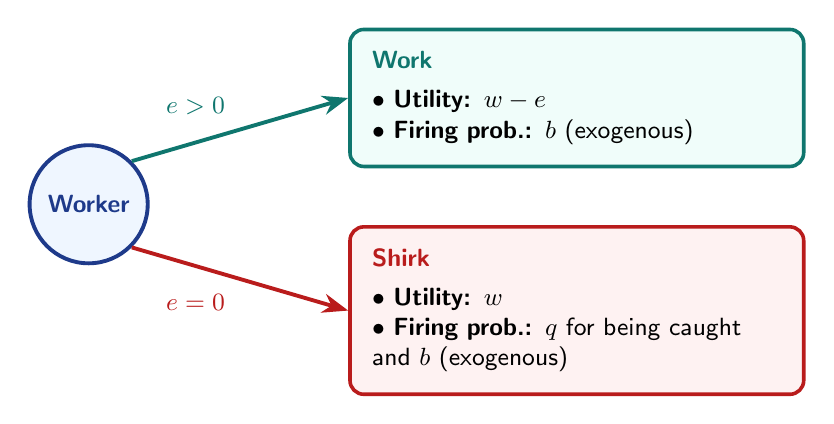
\begin{tikzpicture}[
    >=Stealth,
    font=\sffamily,
    root/.style={
        circle,
        draw=navy,
        line width=1.4pt,
        fill=navylight,
        minimum size=1.5cm,
        align=center,
        font=\sffamily\bfseries\small,
        text=navy
    },
    outcome_work/.style={
        rectangle,
        rounded corners=5pt,
        draw=teal,
        line width=1.3pt,
        fill=teallight,
        text width=5.2cm,
        inner sep=8pt,
        align=left,
        font=\sffamily\small
    },
    outcome_shirk/.style={
        rectangle,
        rounded corners=5pt,
        draw=crimson,
        line width=1.3pt,
        fill=crimsonlight,
        text width=5.2cm,
        inner sep=8pt,
        align=left,
        font=\sffamily\small
    }
]

% Root Decision Node
\node[root] (worker) at (0, 0) {Worker};

% Outcome Nodes
\node[outcome_work] (work) at (6.2, 1.35) {
    \textbf{\textcolor{teal}{Work}} \\[3pt]
    $\bullet$ \textbf{Utility:} $w - e$ \\
    $\bullet$ \textbf{Firing prob.:} $b$ (exogenous)
};

\node[outcome_shirk] (shirk) at (6.2, -1.35) {
    \textbf{\textcolor{crimson}{Shirk}} \\[3pt]
    $\bullet$ \textbf{Utility:} $w$ \\
    $\bullet$ \textbf{Firing prob.:} $q$ for being caught and $b$ (exogenous)
};

% Decision Branches
\draw[->, line width=1.4pt, teal] (worker.north east) -- (work.west)
    node[midway, above left=2pt, font=\sffamily\bfseries\small, text=teal] {$e > 0$};

\draw[->, line width=1.4pt, crimson] (worker.south east) -- (shirk.west)
    node[midway, below left=2pt, font=\sffamily\bfseries\small, text=crimson] {$e = 0$};

\end{tikzpicture}
\end{center}


\end{frame}

\begin{frame}[allowframebreaks]{Asset Equations}
    If she decides to work, her asset equation is given by:
    \begin{equation*}
  \underbrace{rV_E^N}_{\text{Return on Asset}}
  = \underbrace{w - e}_{\text{Flow Benefit}}
  + \underbrace{b(V_u - V_E^N)}_{\text{Expected Capital Loss}}
\end{equation*}
    \begin{itemize}
        \item Probability of being fired: $b$ (exogenous)
        \item Loss: $V_u - V_E^N$
    \end{itemize}
    If she decides to shirk, her asset equation is given by:
    \begin{equation*}
        \underbrace{rV_E^S}_{\text{Return on Asset}} = \underbrace{w}_{\text{Flow Benefit}} + \underbrace{(b + q)(V_u - V_E^S)}_{\text{Expected Capital Loss}}
    \end{equation*}
    \begin{itemize}
        \item Probability of being fired: $b +q$ (exogenous + endogenous)
        \item Loss: $V_u - V_E^S$
    \end{itemize}
    \framebreak
    Finally, if she is unemployed, her asset equation is given by:
    \begin{equation*}
        \underbrace{rV_u}_{\text{Return on Asset}} = \underbrace{\bar{w}}_{\text{Flow Benefit}} + \underbrace{a(V_E - V_u)}_{\text{Expected Capital Gain}}
    \end{equation*}
    \begin{itemize}
        \item Unemployment benefits: $\bar{w}$
        \item Hiring rate: $a$
        \item Gain: $V_E - V_u$ (where $V_E$ is either $V_E^N$ or $V_E^S$ depending on whether the worker will work or shirk after being hired)
    \end{itemize}
\end{frame}

\begin{frame}{No-Shirking Condition}
    In order for a worker to exert effort (not shirk), the following condition must hold:
    $$V_E^N \geq V_E^S$$
    Plugging in the asset equations, we get the \textbf{No-Shirking Condition (NSC)}:
    $$w \ge rV_u + \frac{(r + b + q)e}{q} \equiv \hat{w}$$
    whereby $\hat{w}$ is the \textit{critical wage}.
\end{frame}

\begin{frame}{Firm's Choice}
    \begin{itemize}
        \item If $w < \hat{w}$, workers will shirk due to (1) the low wage $w$ and (2) a high probability $a$ of being rehired (high labor demand at low $w$). $\Rightarrow$ Firm should increase $w$ to $\hat{w}$ to prevent shirking.
        \item If $w > \hat{w}$, workers will exert effort $e$ due to (1) the high wage $w$ and (2) a low probability $a$ of being rehired (low labor demand at high $w$). $\Rightarrow$ Firm should decrease $w$ to $\hat{w}$ to save costs.
    \end{itemize}
    \begin{block}{Conclusion}
        The \textit{NSC} is binding for the firm, i.e. all firms will choose the lowest possible wage that fulfills it, which is $\hat{w}$. They will also pay the minimum unemployment benefits $\bar{w}$ because higher benefits both directly increase costs and increase the \textit{NSC}.
    \end{block}
\end{frame}

\begin{frame}[allowframebreaks]{Aggregate NSC}
    Plugging in the asset equation for unemployed workers $rV_u$, we get the \textbf{Aggregate NSC}:
    $$w \ge \bar{w} + e + \frac{e(a + b + r)}{q}$$
    In steady state, the employment pool $L$ stays constant, i.e. the flow into unemployment must equal the flow out of unemployment:
    $$ bL = a(N-L) \Leftrightarrow a = \frac{bL}{N-L}$$
    where $L$ is the number of employed workers and $N$ is the total number of workers.
    Now plugging steady state $a$ and $V_u$ into the NSC, we get the \textbf{Aggregate Steady-State NSC}:
    $$w \geq e + \bar{w} + \frac{e}{q} \left(\frac{b}{u} + r\right) \equiv \hat{w} \quad \text{where} \ u = \frac{N-L}{N}$$
    \framebreak
    \begin{center}
        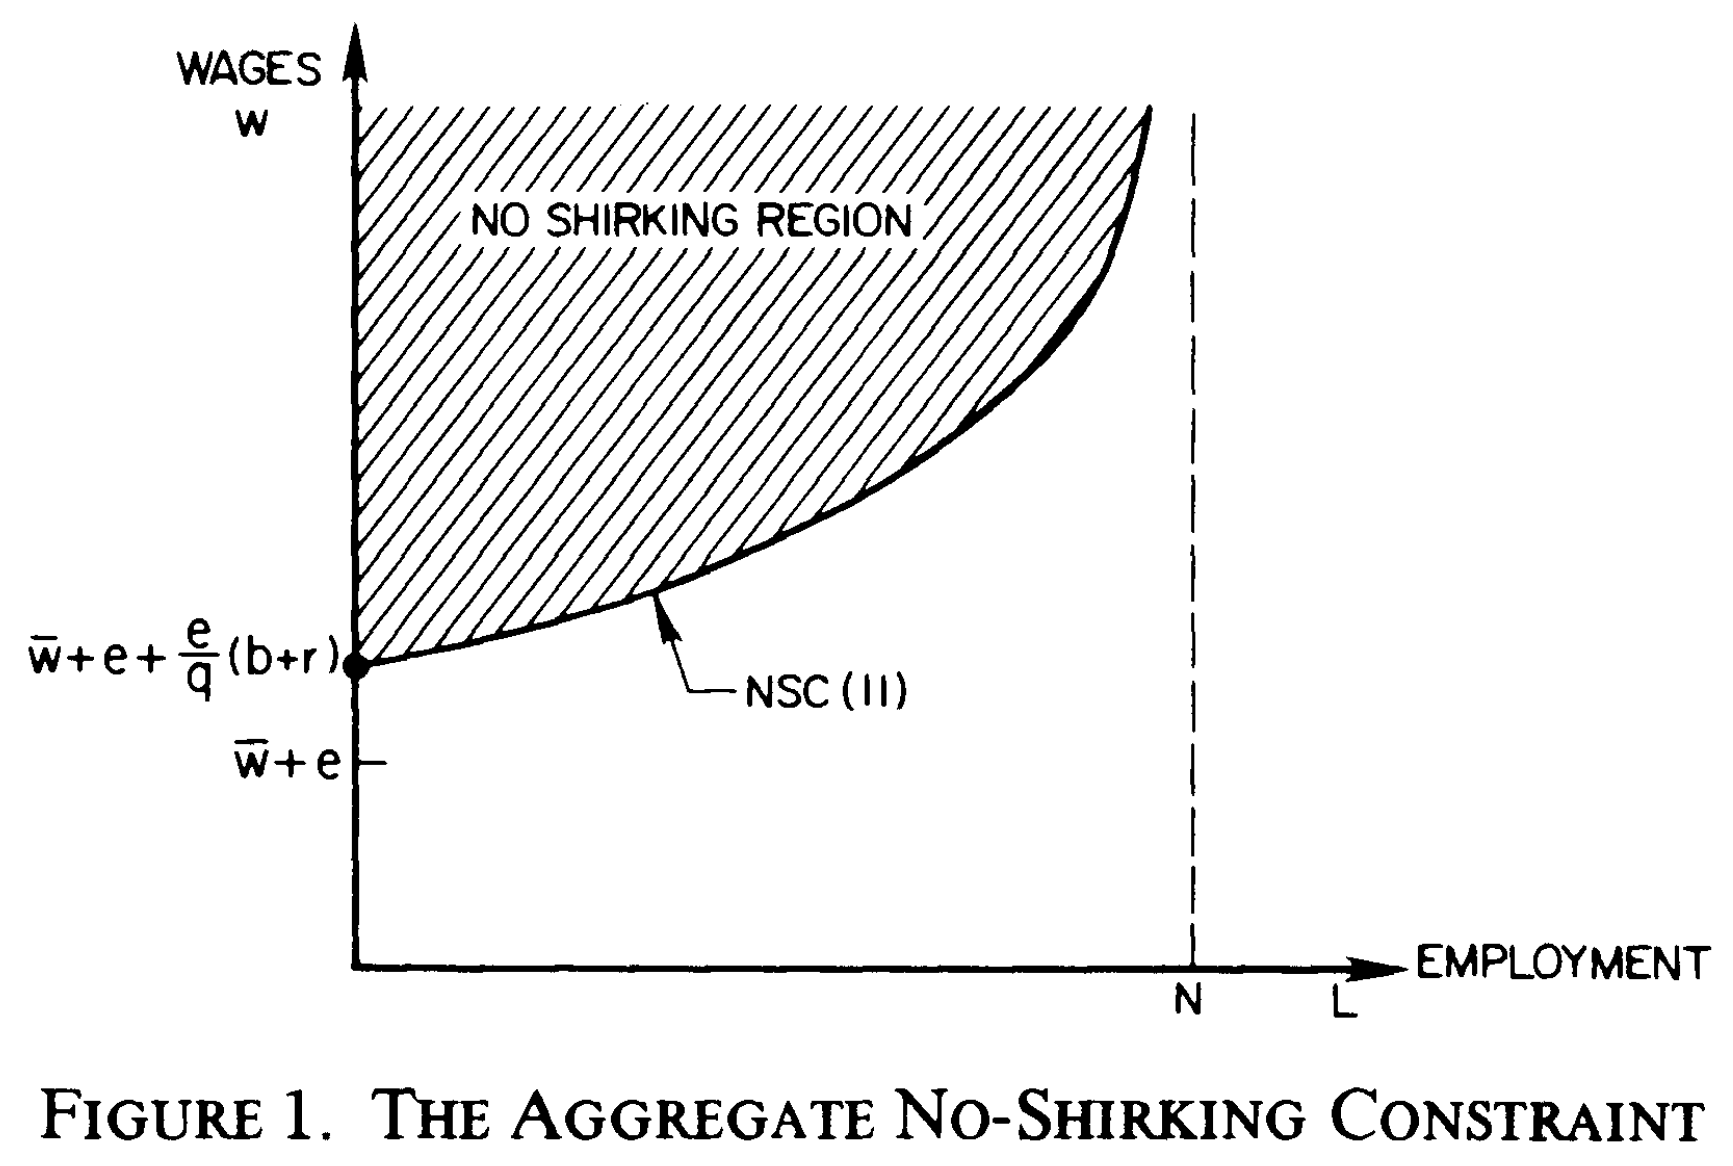
\includegraphics[width=0.8\textwidth]{Figures/agg_NSC.png}
    \end{center}
    
\end{frame}

\begin{frame}{Equilibrium}
    \begin{center}
        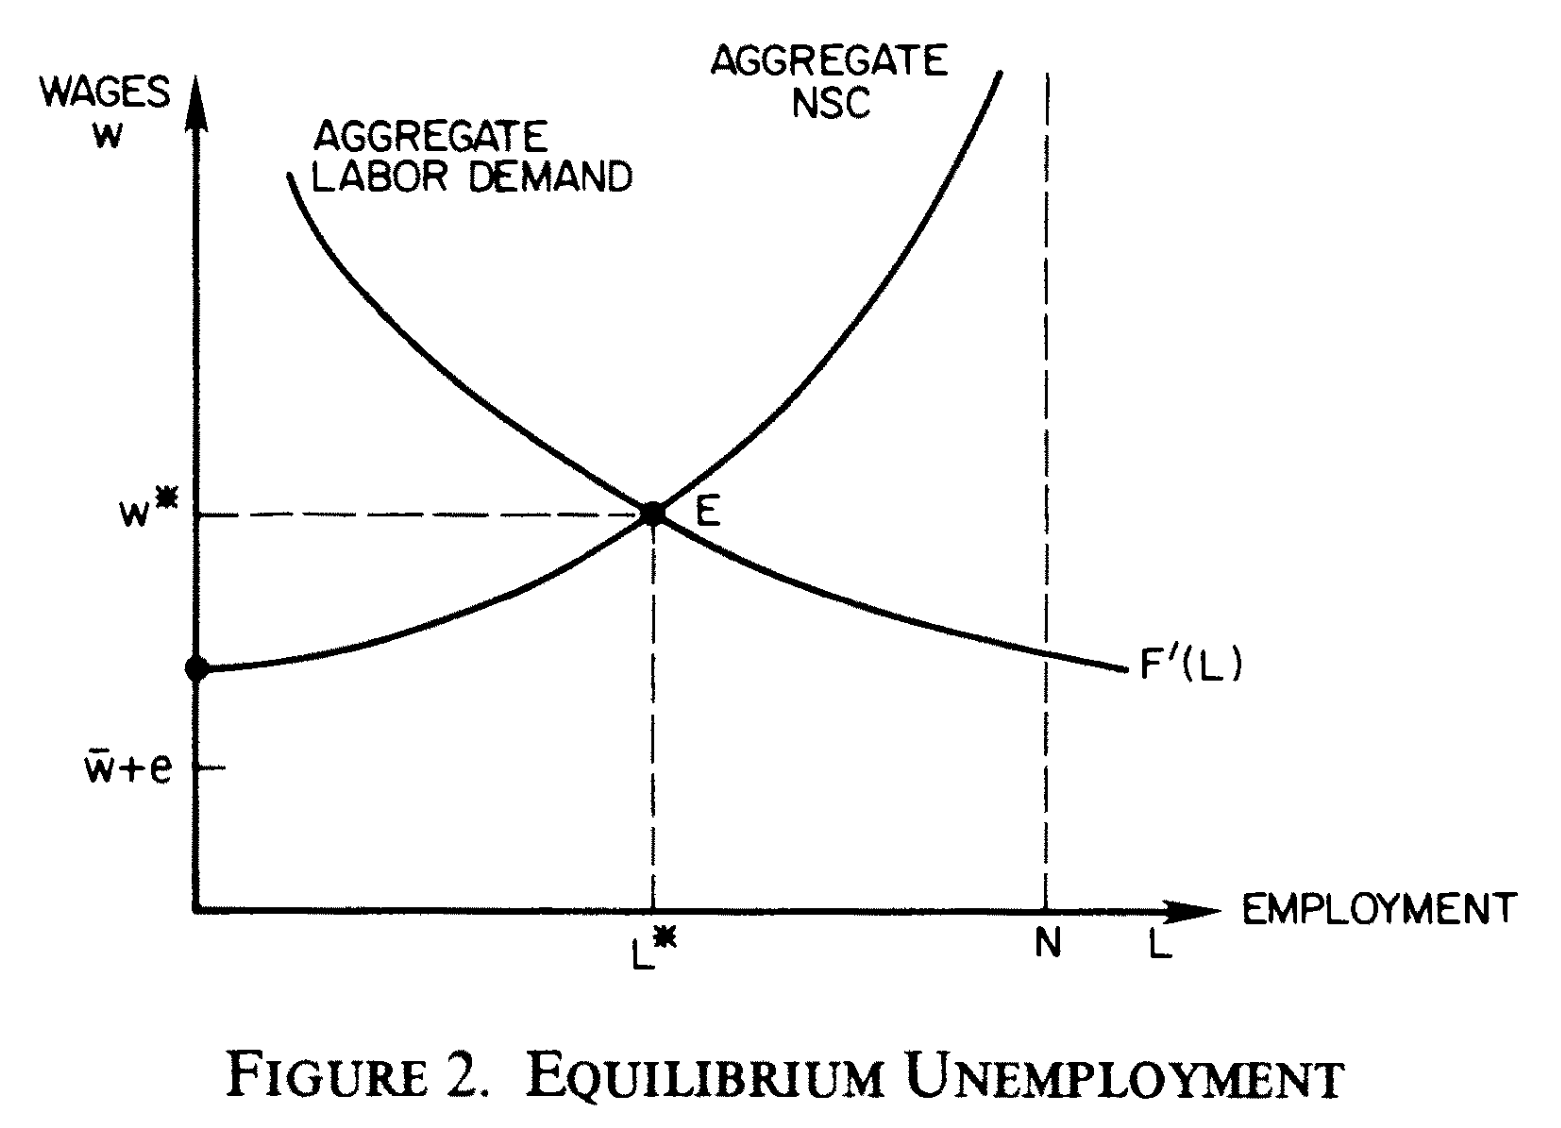
\includegraphics[width=0.8\textwidth]{Figures/Equilibrium.png}
    \end{center}
    
\end{frame}

\begin{frame}{Comparative Statics}
    \centering
    % Left side: The Figure
    \begin{minipage}{0.5\textwidth}
        \centering
        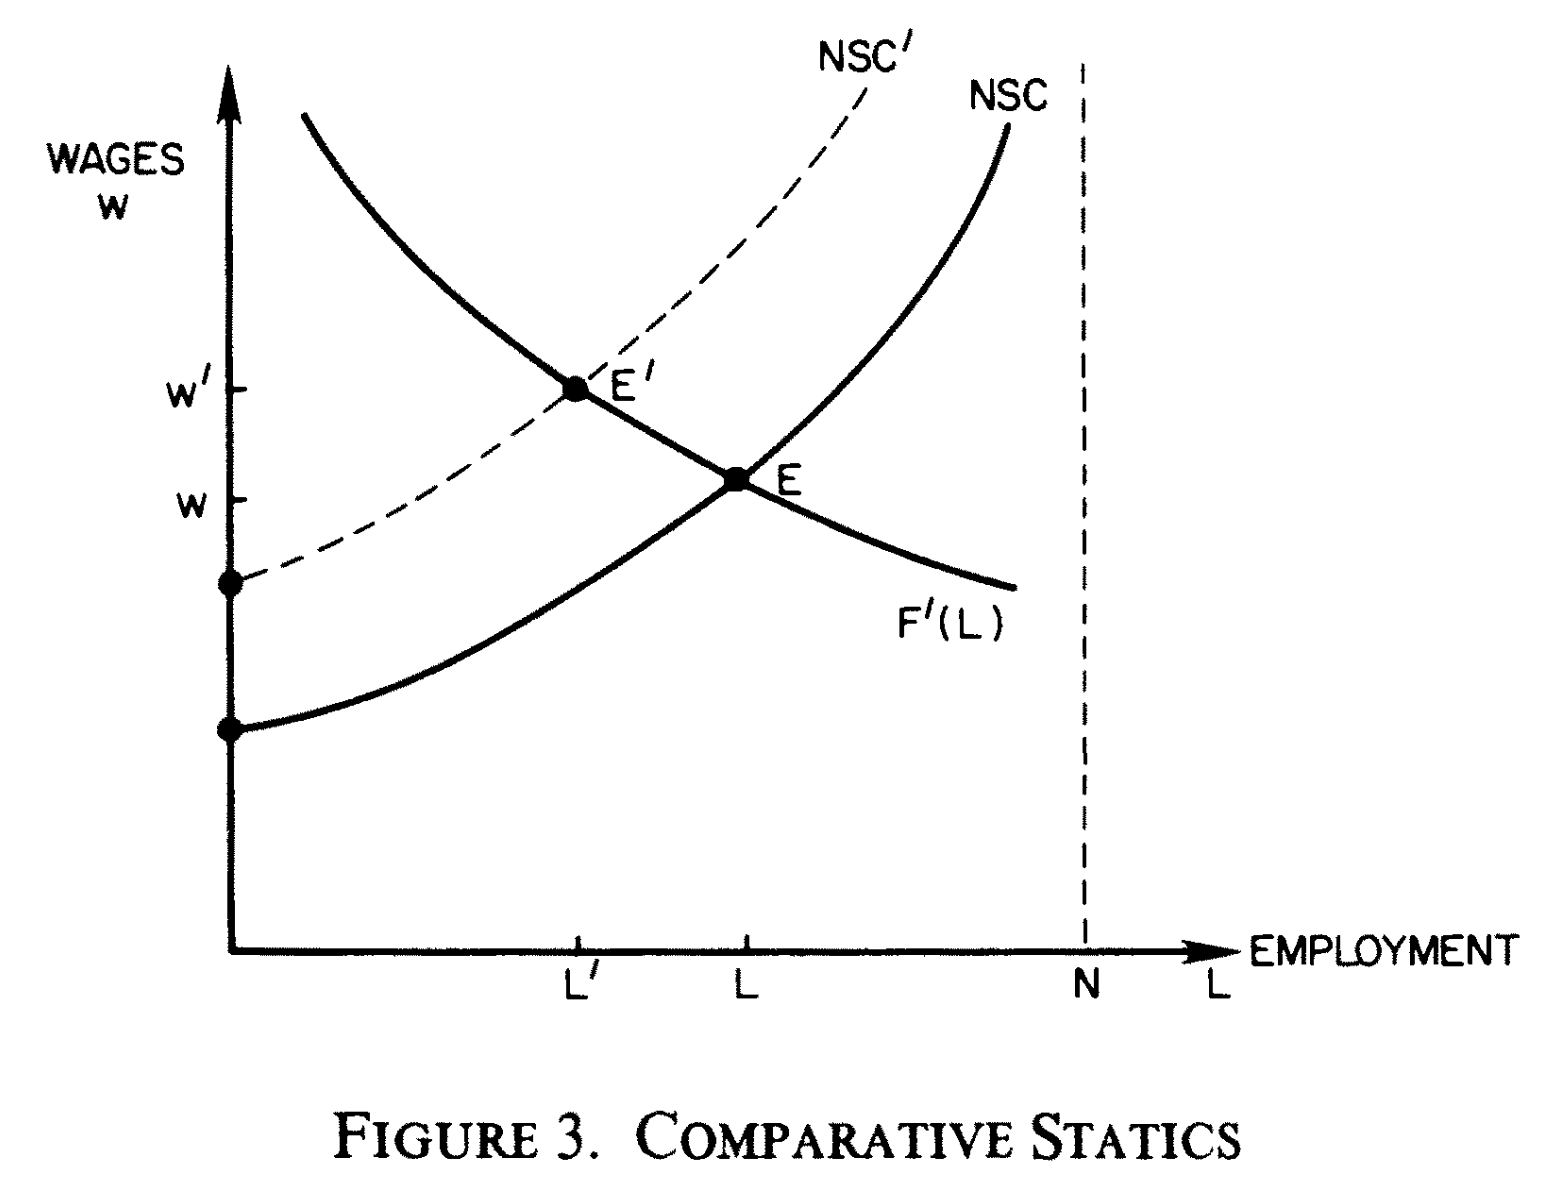
\includegraphics[width=\textwidth]{Figures/Comp_Statics.png}
    \end{minipage}% <--- Note: This percent sign prevents a line break
    \hfill
    % Right side: The Text
    \begin{minipage}{0.45\textwidth}
        NSC shifts up if:
        \begin{itemize}
            \item quit rate $b$ increases
            \item monitoring intensity $q$ decreases
            \item required effort $e$ increases
        \end{itemize}
    \end{minipage}
\end{frame}

\begin{frame}{Welfare Analysis}
    \centering
    % Left side: The Figure
    \begin{minipage}{0.5\textwidth}
        \centering
        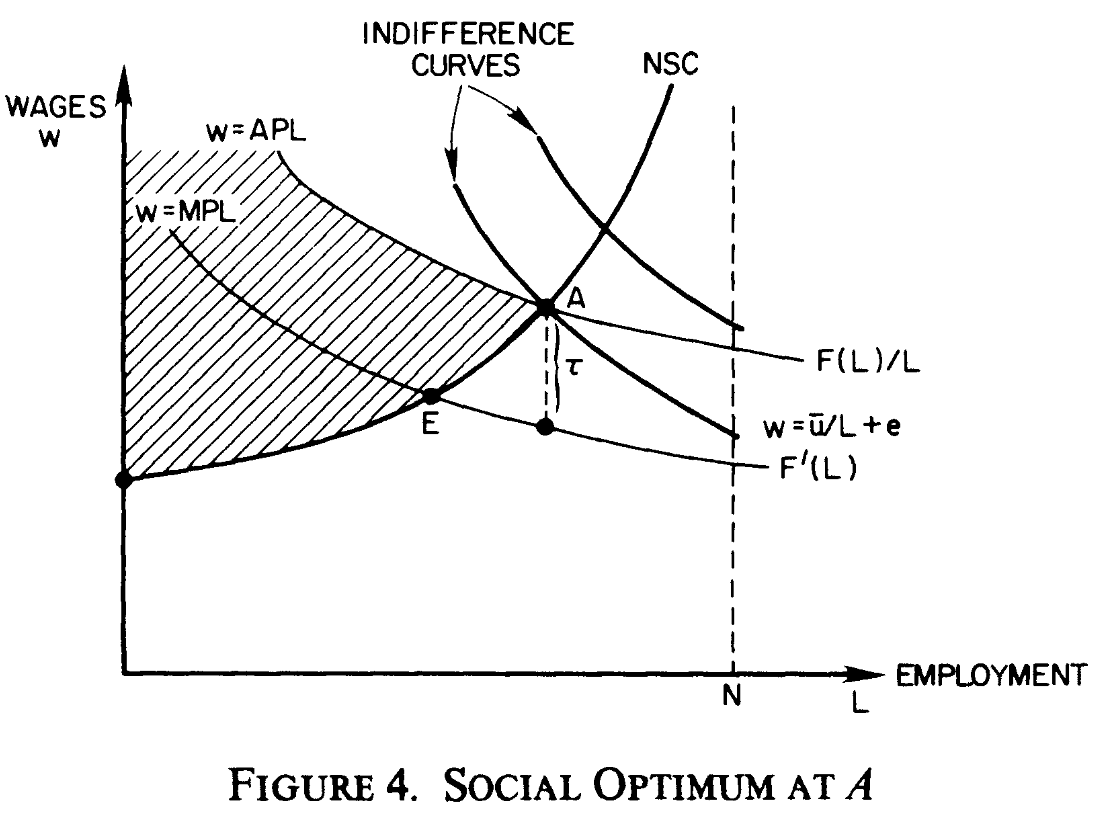
\includegraphics[width=\textwidth]{Figures/Social_Optimum.png}
    \end{minipage}% <--- Note: This percent sign prevents a line break
    \hfill
    % Right side: The Text
    \begin{minipage}{0.45\textwidth}
        A \textit{wage subsidy $\tau$} (financed by taxing away firm profits) could increase aggregate welfare, employment, and production.\par\medskip
        It constitutes a \textit{Pareto improvement} if firms are owned by workers, but not if capital owners and workers are distinct classes.\par\medskip
        \textbf{$\Rightarrow$ No separation between efficiency and income distribution.}

    \end{minipage}
\end{frame}

\begin{frame}{Discussion}
    What should be the minimum requirement for unemployment benefits $\bar{w}$? How does it differ based on the risk profile of workers?\par\medskip
    What alternative discipline devices could be used to reduce shirking?
\end{frame}

\begin{frame}[plain,c]
    \begin{center}
        {\Huge\bfseries Appendix}
    \end{center}
\end{frame}

\begin{frame}{Sluggish Wage Adjustment After a Demand Shock}
\begin{center}
\resizebox{0.82\textwidth}{!}{%
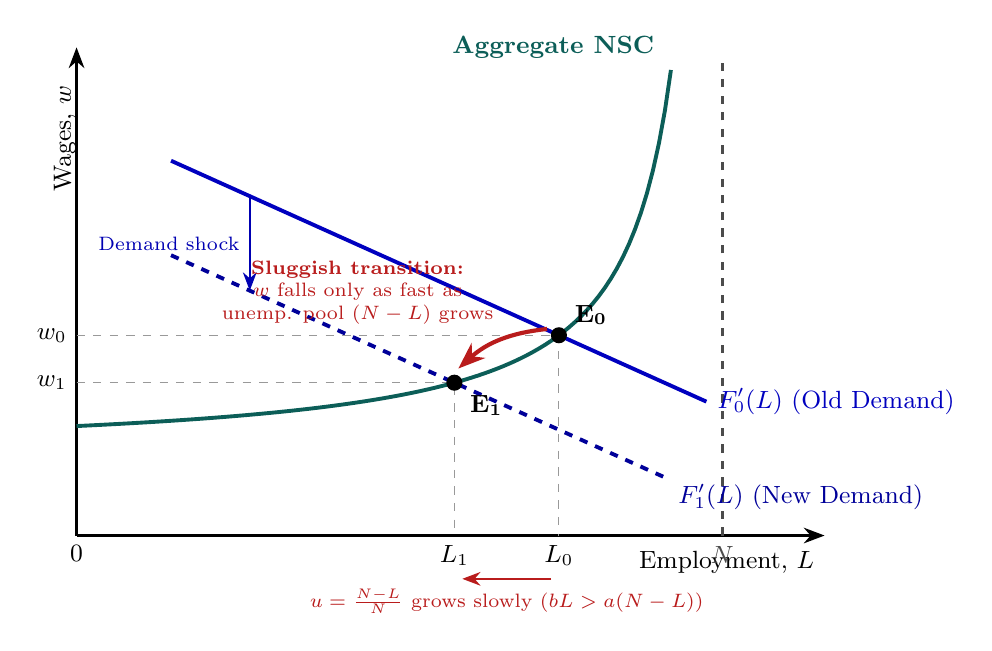
\begin{tikzpicture}[
    >=Stealth,
    thick,
    font=\small,
    curve/.style={line width=1.4pt},
    dashedline/.style={dashed, gray!80, thin}
]
    % Axes
    \draw[->, line width=1pt] (0,0) -- (9.5,0) node[below left, yshift=-2pt] {Employment, $L$};
    \draw[->, line width=1pt] (0,0) -- (0,6.2) node[below left, rotate=90, yshift=12pt, xshift=-10pt] {Wages, $w$};

    % Full Employment Asymptote (N)
    \draw[dashed, black!70, line width=1pt] (8.2,0) node[below] {$N$} -- (8.2,6.0);
    \node[below] at (0,0) {$0$};

    % 1. Aggregate NSC Curve: w = e + w_bar + (e/q)*(bN/(N-L) + r)
    \draw[curve, teal!80!black, domain=0:7.55, samples=100, name path=nsc]
        plot (\x, {1.0 + 3.2/(8.2 - \x)}) node[above left, xshift=-2pt] {\textbf{Aggregate NSC}};

    % 2. Old Labor Demand Curve F'_0(L)
    \draw[curve, blue!75!black, domain=1.2:8.0, samples=50, name path=ld0]
        plot (\x, {5.3 - 0.45*\x}) node[right] {$F'_0(L)$ (Old Demand)};

    % 3. New Labor Demand Curve F'_1(L)
    \draw[curve, blue!60!black, dashed, domain=1.2:7.5, samples=50, name path=ld1]
        plot (\x, {4.1 - 0.45*\x}) node[below right, yshift=2pt] {$F'_1(L)$ (New Demand)};

    % Exact intersections for E_0 and E_1
    \path[name intersections={of=nsc and ld0, by=E0}];
    \path[name intersections={of=nsc and ld1, by=E1}];

    \coordinate (E0_y) at (0,0 |- E0);
    \coordinate (E1_y) at (0,0 |- E1);
    \coordinate (E0_x) at (0,0 -| E0);
    \coordinate (E1_x) at (0,0 -| E1);

    % Dashed projection lines
    \draw[dashedline] (E0_y) node[left, black] {$w_0$} -- (E0) -- (E0_x) node[below, black] {$L_0$};
    \draw[dashedline] (E1_y) node[left, black] {$w_1$} -- (E1) -- (E1_x) node[below, black] {$L_1$};

    % Demand shift arrow
    \draw[->, blue!70!black, thick] (2.2, 4.31) -- node[left, font=\scriptsize] {Demand shock} (2.2, 3.11);

    % Sluggish adjustment arrow along the NSC as unemployment pool grows
    \draw[->, crimson, line width=1.5pt, bend right=18]
        ($(E0) + (-0.15, 0.08)$) to node[above left, font=\scriptsize, align=center, xshift=2pt, yshift=2pt]
        {\textbf{Sluggish transition:}\\$w$ falls only as fast as\\unemp. pool $(N-L)$ grows}
        ($(E1) + (0.05, 0.18)$);

    % Bottom bracket showing unemployment pool growth
    \draw[->, crimson, thick] ($(E0_x) + (-0.1, -0.55)$) -- node[below, font=\scriptsize] {$u = \frac{N-L}{N}$ grows slowly ($bL > a(N-L)$)} ($(E1_x) + (0.1, -0.55)$);

    % Plot Equilibrium Points
    \filldraw[black] (E0) circle (2.5pt) node[above right, xshift=2pt] {$\mathbf{E_0}$};
    \filldraw[black] (E1) circle (2.5pt) node[below right, xshift=2pt, yshift=-1pt] {$\mathbf{E_1}$};

\end{tikzpicture}
}%
\end{center}
\end{frame}

\end{document}
